\chapter{Tutorial 1: the absorption spectrum of pyrene at 0~K}\label{ch:tut-pyrene}

This tutorial computes the absorption spectrum of pyrene
(C$_{16}$H$_{10}$, 72 modes) from the ground state, with the DFT
quartic force field of the reference test case.
% TODO(maintainer): level of theory of the pyrene force field.
The input files are in \file{examples/pyrene}; the same force field is published in the PAH
database of INAF--OACa, \url{https://cosmicpah-qcals.oa-cagliari.inaf.it}.

\section{Input files}

\begin{description}
\item[\file{freqsfile}] One line per mode: harmonic wavenumber (cm$^{-1}$)
  and the three components of $\partial\mu/\partial q$ (atomic units).
\item[\file{phi3file}, \file{phi4file}] Cubic and quartic force constants
  (cm$^{-1}$, dimensionless normal coordinates), one per line, with 1-based
  indices.
\item[\file{dmu2file}] Second derivatives of the dipole (a.u.).
\item[\file{quantafile}] The starting states: one line per state, with the
  quantum numbers of all the modes and a repetition count. Here it contains
  only the ground state.
\item[\file{inp}] The options (Section~\ref{sec:inp}). The essential ones for this tutorial:
\end{description}
\begin{lstlisting}
nmodes = 72
fermithres = 0.20        # resonance thresholds (|W/D|)
ddthres = 0.20
hsizescalepar = 8        # polyad size
maxtothops = 4
bandthres = 1e-3         # which overtone/combination bands to compute
eigensolver = 2          # ScaLAPACK (see below)
computeground = 1
wnumhistmin = 0          # spectral grid (cm-1)
wnumhistmax = 9000
wnumhiststep = 0.01
modepopfile = "quantafile"
\end{lstlisting}

\section{Running}

\begin{lstlisting}
thermal_anharmonicity_fase1 > fase1.log
thermal_anharmonicity_fase2a > fase2a.log
mpirun -np 4 thermal_anharmonicity_fase2b > fase2b.log
\end{lstlisting}
(\file{run.sh} does the same, and keeps a copy of \file{out.oct} after each
phase: \file{out.fase1.oct}, \file{out.fase2a.oct}, \file{out.fase2b.oct}.)
The two thresholds can also be set from one variable,
\begin{lstlisting}
thres = 0.20
fermithres = thres
ddthres = thres
\end{lstlisting}
which is handy when testing how the results depend on them.
\file{run.sh} takes about 1 min 40~s on a 4-core laptop: phase 1 about
20~s, phase 2a 4~s, phase 2b about 70~s. Phase 1 finds 1785 resonances
(1609 E4, 89 B3, 79 D4, 8 G2) and writes \file{bandlist} with 31
fundamentals (the modes with a nonzero dipole derivative) and 1264
overtone, combination and difference bands. The largest polyad has 2363
states. (With \opt{minhopcoupling}~$=0$, the default of 2026.11, it has
3582 and phase 2b takes about four times longer.)

Phase 1 prints two warnings:
\begin{lstlisting}
Warning: rotatedcomp is 0.580081>.5 for vib mode 0, possible intensity inaccuracy
  largest term: B3 1 56 56 (1-based, 1 <-> 56 + 56), |Phi/Delta| = 0.611823,
  harmonic Delta = -54.391 cm-1, treated as nonresonant; see rescandfile, resonanceoverrides
\end{lstlisting}
and the same for mode~1 (modes are counted from 0 here, from 1 in the
second line). They are expected. The two highest CH stretches are mixed
strongly by the contact transformation (\texttt{rotatedcomp} above 0.5),
mostly through a Fermi term with the overtone or a combination of mode~56
(the second line names it), which the default criterion treats as
nonresonant; so their intensities, computed perturbatively, are less
accurate (Chapter~\ref{ch:trouble}). Tutorial~4
(Chapter~\ref{ch:tut-review}) shows how to review such terms, and with
\opt{rescriterion}~$=1$ they are treated as resonant and the warnings
disappear.

\section{What to look at}

\begin{itemize}
\item \file{resonanceslist}: the Fermi (B3) and Darling--Dennison (E4, D4)
  resonances.
\item \file{dunhamparams}: the deperturbed fundamentals $\nu_i$ and
  anharmonic constants $x_{ij}$.
\item The histograms \file{hist\_abs\_0}, \file{\_1} and \file{\_2}: the
  $x$, $y$ and $z$ components of the absorption spectrum.
\end{itemize}

The script \file{plot\_spectrum.py} (in \file{examples/pyrene}, needs numpy
and, for the figure, matplotlib) adds the three components, converts them to
integrated intensities in km/mol ($I = 16.194\,\tilde\nu\,|\mu|^2$, with
$|\mu|^2$ in atomic units as stored in the histograms), lists the strongest
lines and draws Figure~\ref{fig:pyrene}:
\begin{lstlisting}
python3 plot_spectrum.py . 8
\end{lstlisting}
The run gives 3963 lines with a total of 446.1~km/mol. The strongest are:
\begin{center}
\begin{tabular}{rr}
\toprule
wavenumber (cm$^{-1}$) & intensity (km/mol) \\
\midrule
844.79 & 109.92 \\
711.91 & 43.95 \\
3035.46 & 38.69 \\
742.61 & 16.00 \\
3037.83 & 14.11 \\
1184.00 & 12.16 \\
202.22 & 10.19 \\
3042.34 & 9.97 \\
\bottomrule
\end{tabular}
\end{center}

\begin{figure}[htbp]
\centering
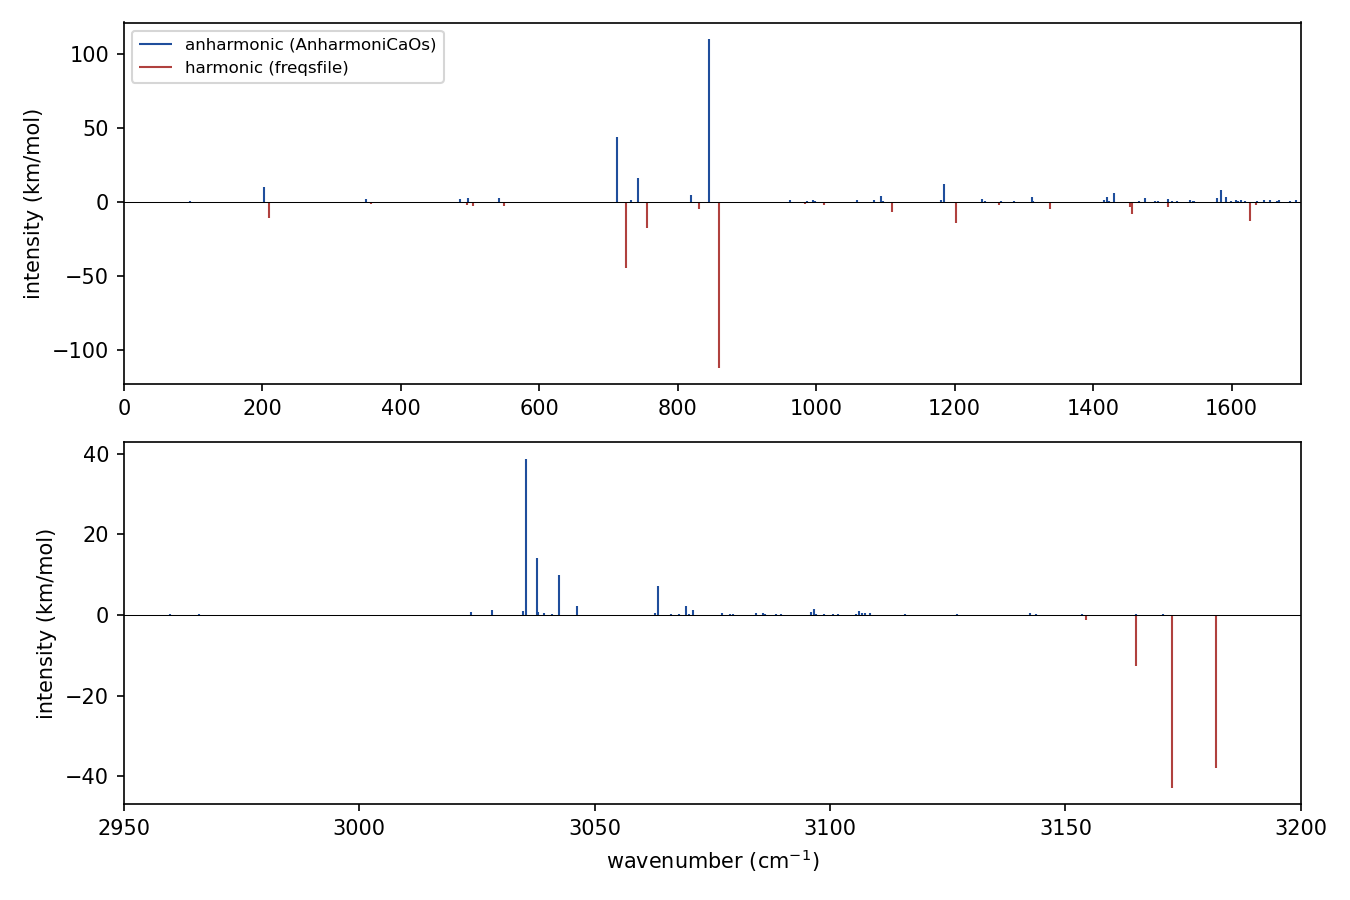
\includegraphics[width=\textwidth]{figures/pyrene-spectrum.png}
\caption{Pyrene, absorption from the ground state: the lines computed in
this tutorial (up) against the harmonic fundamentals of \file{freqsfile}
(down). The CH stretches (lower panel) move down by about 140~cm$^{-1}$ and
split among the states they are in resonance with.}
\label{fig:pyrene}
\end{figure}

These numbers and the figure come from a run of \file{run.sh} with
AnharmoniCaOs 2026.11.1 (\texttt{git 88b3b13}, the release candidate; the
programs of the release are the same) on a 4-core laptop.

\subsection*{Choice of the eigensolver}

\opt{eigensolver} selects the library that diagonalises the polyads in
phase 2b:
\begin{itemize}
\item \texttt{2}, ScaLAPACK \texttt{pdsyevx}: used in all the tutorials;
\item \texttt{1}, ScaLAPACK \texttt{pdsyevr}: same spectra;
\item \texttt{0}, SLEPc: the lines it finds agree with ScaLAPACK, but
  some weak lines are missing (on the same input with \opt{hsizescalepar}~=~4,
  1439 lines and 2\% of the total intensity); the reason is being
  investigated;
\item \texttt{3}, ELPA: same spectra (relative L1 distance below
  $10^{-7}$, the same transition energies), and the fastest. Its two-stage
  solver (\opt{elpasolver}~=~2) needs blocks of at most 64
  (\opt{elpablock}); with blocks of 300 it gave wrong eigenvalues on the
  polyads of 3400 states and more, without any error.
\end{itemize}

Wall time of phase 2b of this tutorial on a 4-core laptop, with
AnharmoniCaOs 2026.11.1 (\texttt{git 88b3b13}); the three runs give the
same total, 446.08~km/mol:
\begin{center}
\begin{tabular}{lrr}
\hline
eigensolver & processes $\times$ threads & wall time \\
\hline
\texttt{pdsyevx} (2) & $4\times1$ & 1:05 \\
ELPA one-stage (3) & $1\times1$ & 0:27 \\
\opt{spectral}~$=1$, \opt{spectralexactmax}~$=3000$ & $1\times4$ & 0:06 \\
\hline
\end{tabular}
\end{center}
On polyads of this size more processes do not help: the cost of
distributing the matrices exceeds the gain, and one process with ELPA, or
several independent runs, is the efficient choice. The spectral method
(option \opt{spectral}) is fastest; with \opt{spectralexactmax} as
large as the largest polyad all the polyads are diagonalised exactly and
the spectrum agrees with the other solvers within its resolution
(relative L1 distance 0.5\%).

\section{Variations}

The same run with the options of Chapter~\ref{ch:inputs}:
\begin{itemize}
\item \opt{shiftgeometry}: lines shift by up to about 3~cm$^{-1}$, and some
  intensities change by 10--30\%;
\item \opt{closureterms}: only weak lines change;
\item \opt{dipole3}: the CH stretches go from 7.5\% to 10.3\% of the total
  intensity.
\end{itemize}
